\documentclass{article}
\usepackage{geometry}
\usepackage{paralist}
\usepackage[T1]{fontenc}
\usepackage{reledmac}
\usepackage{changepage}
\usepackage{layout}

\usepackage{pgfplots}
\usepackage{tikz}
\usetikzlibrary{positioning}
\usetikzlibrary{shapes.geometric, arrows}
\usetikzlibrary{calc, shapes, backgrounds}
\tikzstyle{arrow} = [thick,->,>=stealth]

\usepackage{graphicx} 
\graphicspath{ {./images/} }

\usepackage{fancyhdr}
\fancyhead[L]{
	\begin{tabular}{l}
		\Large \textbf{\textsc{Distributed Systems}} \\
		\large Project 02 - Part 02
	\end{tabular}
}
\fancyhead[R]{
	\begin{tabular}{r}
		16-124-836 \\
		Marcel \textsc{Zauder}
	\end{tabular}
}
\renewcommand{\headrulewidth}{0.4pt}
\fancyfoot[C]{\thepage}
\renewcommand{\footrulewidth}{0.4pt}
\setlength{\headsep}{35pt}
\setlength{\textheight}{600pt}

\usepackage{hyperref}

\begin{document}
	\pagestyle{fancy}
	
	All required files are in their respective directories with specified names.	
	
	\section*{Task 08 - Redis-Benchmark}
	\begin{adjustwidth}{2em}{2em}
		For each benchmark test in Task 8.1, 8.2, and 8.3 I used the command: \\
		\begin{adjustwidth}{-2em}{-2em}
		\small{\emph{\textit{redis-benchmark -t set,lpush,get,lpop -n 100000 -q -h ThunderStorm\_server-\$NEED\_UUID (> benchmark.txt)}}}
		\end{adjustwidth}
		\hfill \\
		When running the redis benchmark with the simple\_topology, we get approximately 997 requests per second for each command (\textsc{set, lpush, get, lpop}). When increasing the bandwidth in Task 8.2 the amount of requests per second do not increase which means this amount is not dependent on the bandwidth but on the latency. This can also be approved by computation because when using the double round trip time of 50ms in both topologies and know that each packet consists of 50 requests, we get approximately 1000 packets which should be sent in one second which is also the amount we get when running the benchmark test. \\
		When introducing a new client which is directly connected to switch 2 the amount of request per second sent from client 1 is not changing significantly. The amount of requests per second from client 2 is approximately 1200-1250 which is due to the lower latency (40ms for round trip latency) which is also what we would expect when computing this amount ($\frac{40}{50} \times 1000 = 1200$). \\
		In Task 8.3 I used the drop rates 0.001, 0.01, 0.1, and 0.5. With these we get the following plot for requests per second from  client 2: \\
		\begin{center}
			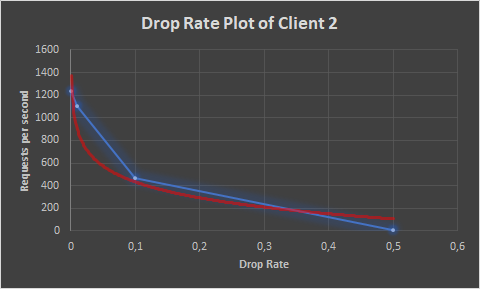
\includegraphics[scale=0.7]{drop_rate.png}
		\end{center}
		\hfill \\
		We can see that the amount of request per second is decreasing somewhat logarithmically such that a low change of a very small drop rate can lead to a huge decrease of requests per second. But the higher it gets the less significant the effect of a small change in the drop rate is.
	\end{adjustwidth}
	\newpage
	\section*{Task 09 - Dynamic Topologies}
	\begin{adjustwidth}{2em}{2em}
		For the benchmark we get the following plot:
	\end{adjustwidth}
	\begin{adjustwidth}{-4em}{}
		\begin{center}
			\includegraphics[scale=0.55]{tha_plot.jpg}
		\end{center}
	\end{adjustwidth}
	\begin{adjustwidth}{2em}{2em}
		The blue graph until the first red line does not matter at all for the actual task, because there was a 120 second lead time, because I needed time to set everything up but the topology is starting as soon as the \texttt{docker stack} command is run. Therefore the benchmark started a bit earlier than we needed it to be. But yet in this part of the graph there are some spikes which can be explained by the blue line being the average of the requests per second and at theses exact points of time ($\sim$ 20 and 40 seconds in the plot) the program is returning the average requests per second (can be also seen in the data when there is the string \textit{SET: 4902,98 requests per second} and sets this average to 0 and therefore the spikes occur. \\
		For the first 10 seconds the average requests per second do not change. As soon as the first change (second red line - latency is increased to 50 ms) occurs the average requests per second is decreasing slowly. The green line shows the approximate amount of requests per second which is instantly dropping to a value of around 900 (this is only an approximation by me because it is the most plausible value for me). While the average requests is decreasing also the bandwidth is decreased (3rd red line) but as also seed in the previous task a change of bandwidth does not affect the amount of requests sent and therefore the graph is not affected as well. At second 95 the code is again returning the current value for the average amount of requests per second and resets the value, therefore the spike. After this the value is pretty much constant at 900 requests per second (therefore my assumption that the amount of requests per second at a latency of 50ms is aroung 900). Again when changing the bandwidth (at the 4th red line to 150Mbps) the average requests per second is not affected. As soon as the latency is increased at the fifth red line to 10ms the number of requests per second is increasing. Again I assumed that overall the requests per second is increased to a value of approximately 3300. The last jump of the plot can be explained by the code having returned and again reset it to 0. \\
		With this whole plot we can again see that only a change in the latency is also changing the amount of requests per second and only a very huge decrease in the bandwidth would have an effect on this value.
	\end{adjustwidth}
\end{document}